In nature world there is no source of parallel ray. Each beams of lights can be in some ways considered from a simple origin: point light source,which emits light in all directions. Thus a normal light source can not provide a perfect focused beams for optical applications. Laser light (laser radiation)has some very special properties, which very much distinguish it from light with other origins:

\begin{itemize}
\item Laser light is usually delivered in the form of a laser beam, i.e. it propagates dominantly in a well-defined direction with moderate beam divergence. Such a laser beam has a high (sometimes extremely high) degree of spatial coherence. This means that the electric fields at different locations across a beam profile oscillate with a rigid phase relationship. Exactly this coherence is the reason why a laser beam can propagate over long distances without spreading very much in the transverse directions, and why it can be focused to very small spots (high focusability of laser beams).

\item In many but not all cases, laser light also has a high degree of temporal coherence, which is equivalent to a long coherence length. This means that a rigid phase relationship is also maintained over relatively long time intervals, corresponding to large propagation distances (often many kilometers) or to huge numbers of oscillation cycles.
\item The large temporal coherence, quantified with a large coherence time or coherence length, is associated with a narrow spectral bandwidth (or linewidth). (We exclude here the sophisticated case of trains of ultrashort pulses, which can have a large optical bandwidth but nevertheless a high degree of coherence; see the article on coherence for details.) For a visible laser beam, this means that it has a certain pure color, e.g. red, green or blue, but not white or magenta. Some lasers allow a degree of wavelength tuning (e.g. dye lasers). The large coherence length introduces a tendency for the phenomenon of laser speckle, i.e. a characteristic granular pattern which can be observed e.g. when the laser beam hits a metallic surface.

\item In most cases, laser light is linearly polarized. This means that the electric field oscillates in a particular spatial direction (? polarization of laser emission).
\end{itemize}

Optical engineers and researchers working on optics 


 %light beams where the electric field profile in a plane perpendicular to the beam axis can be described with a Gaussian function, possibly with an added parabolic phase profile
To undersstand the behavior of laser beams in optics system some characteristics are in following  introduced. 

In optics and particularly in laser physics, laser beams often occur in the form of Gaussian beams, which are named after the mathematician and physicist Johann Carl Friedrich Gau�. Here, the transverse profile of the optical intensity of the beam with a power $P$ can be described with a Gaussian function:

\begin{align}
I(r,z)&=\frac{P}{\pi w(z)^2 /2}exp(-2\frac{r^2}{w(z)^2})
\end{align}


where the beam radius w(z) is the distance from the beam axis where the intensity drops to $1/e2 (\sim13.5\%)$ of the maximum value. A hard aperture with radius w can transmit $\sim86.5\%$ of the optical power. For an aperture radius of $1.5 w$ or $2 w$, this fraction is increased to $98.9\%$ and $99.97\%$, respectively.

In addition to the Gaussian shape of the intensity profile, a Gaussian beam has a transverse phase profile which can be described with a polynomial of at most second order. A linear phase variation in one direction (not considered further here) describes a tilt, and a quadratic phase variation is associated with divergence or convergence of the beam.


Gaussian beams are usually considered in situations where the beam divergence is relatively small, so that the so-called paraxial approximation can be applied. This approximation allows the omission of the term with the second-order derivative in the propagation equation (as derived from Maxwell's equations), so that a first-order differential equation results. Within this approximation, a Gaussian beam propagating in free space remains Gaussian, except that of course its parameters evolve. For a monochromatic beam, propagating in the $z$ direction with the wavelength $\lambda$, the complex electric field amplitude (phasor) is
\begin{align}
E(r,z) =E_{0}\frac{w_{0}}{w(z)}exp(-2\frac{r^2}{w(z)^2})exp(-i[kz-arctan\frac{z}{z_{R}}+\frac{kr^2}{2R(z)}])
\end{align}

with the peak amplitude $|E0|$ and beam radius w0 at the beam waist, the wavenumber $k = 2\pi /\lambda$, the Rayleigh length $z_{R}$ (see below) and the radius of curvature $R(z)$ of the wavefronts. The oscillating real electric field is obtained by multiplying the phasor with $exp(i 2\pi ct/ \lambda)$ and taking the real part.

\begin{figure}
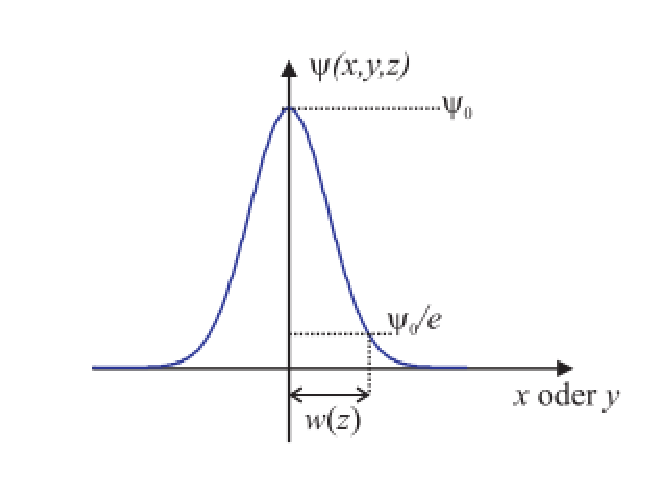
\includegraphics[width=0.8\textwidth]{bilder/gussian_verteilung}
\caption{Transversal profie of the Gussian beam amplitude at the beam waist (dashed line) and irradiance (solid line). Both of them have been normalized to the maximum value. The value of the width of the beam waist $\omega_{0}$ is 0.1 mm. The horizontal lines represent  (in increasing value)the $1/e^{2}$ of the maximum irradiance, the $1/e$ of the maximum amplitude, and the 0.5 of the maximum irrance and amplitude.}
\label{fig:gussian_verteilung}
\end{figure}
%Spot Size
One of important characters is \textbf{Spot Size}.In a cross-section of a gaussian beam the beam intesity is approximately distibuted as gaussian function. The spot size is the diameter of a area at whose edge the value of the electrical field intensity decay to $1/e$ of its peak value, otherwise the energy density to $1/e^2$ of the peak value. 


More detail information about gaussian beam can be found in \cite{laser_gaussianbeam_propagation}\cite{script_FT_TET}\cite{CVI_Melles_Griot_Technical_Guide}.